%!TEX root = ../../thesis.tex

Experimental signatures for the Higgs boson are categorised according to production 
mode and decay channel.

In a hadron collider such as the \ac{LHC}, the important production modes are \ac{ggF},
\ac{VBF}, Higgs-strahlung and top fusion. \Figure~\ref{fig:feyn} displays Feynman diagrams 
of each. As gluons are massless and the Higgs boson couples to mass, \ac{ggF} proceeds via 
loops of massive coloured particles (predominantly the top quark owing to its large mass). 
The other three modes feature additional final state particles which can aid 
identification. In particular, \ac{VBF} has two back-to-back quarks with no colour 
exchange between them. The production cross sections at the \ac{LHC} are shown in
\Figure~\ref{fig:higgs_xs}, for a \ac{CM} energy of \unit{8}{\TeV} and a range of \mH.

\begin{figure}
	\null\hfill
	\begin{subfigure}[b]{0.4\textwidth}
		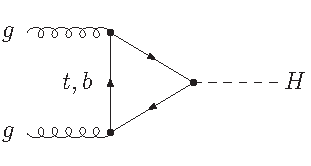
\includegraphics[width=\textwidth]{axodraw/ggF.pdf}
		\caption{Gluon-gluon fusion}
		\label{fig:feyn:ggF}
	\end{subfigure}
	\hfill
	\begin{subfigure}[b]{0.3\textwidth}
		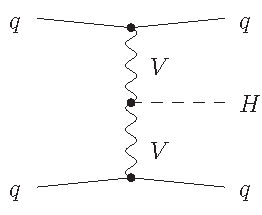
\includegraphics[width=\textwidth]{axodraw/VBF.pdf}
		\caption{Vector boson fusion}
		\label{fig:feyn:VBF}
	\end{subfigure}
	\hfill\null
	\\\bigskip
	\null\hfill
	\begin{subfigure}[b]{0.33\textwidth}
		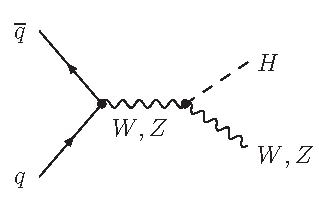
\includegraphics[width=\textwidth]{axodraw/VH.pdf}
		\caption{Higgs-strahlung}
		\label{fig:feyn:VH}
	\end{subfigure}
	\hfill
	\begin{subfigure}[b]{0.25\textwidth}
		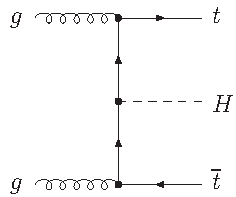
\includegraphics[width=\textwidth]{axodraw/ttH.pdf}
		\caption{Top fusion}
		\label{fig:feyn:ttH}
	\end{subfigure}
	\hfill\null
	\caption{Examples of tree-level Feynman diagrams for the Higgs production processes relevant at the \ac{LHC}.}
	\label{fig:feyn}
\end{figure}

\begin{figure}
	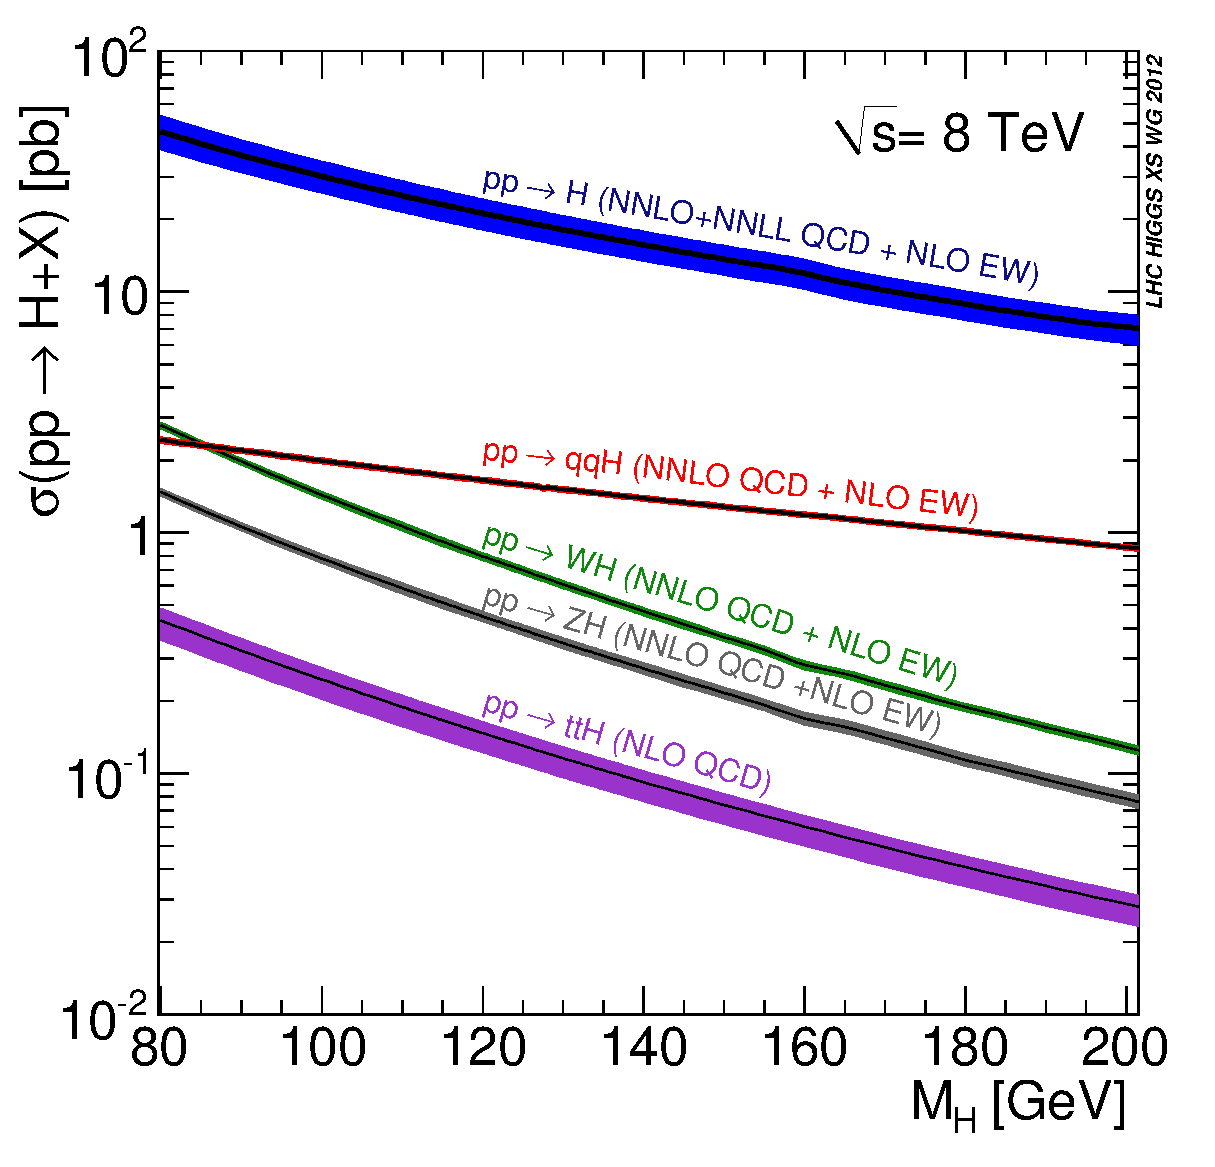
\includegraphics[width=0.48\textwidth]{tex/motivation/xs_lowrange}
	\hfill
	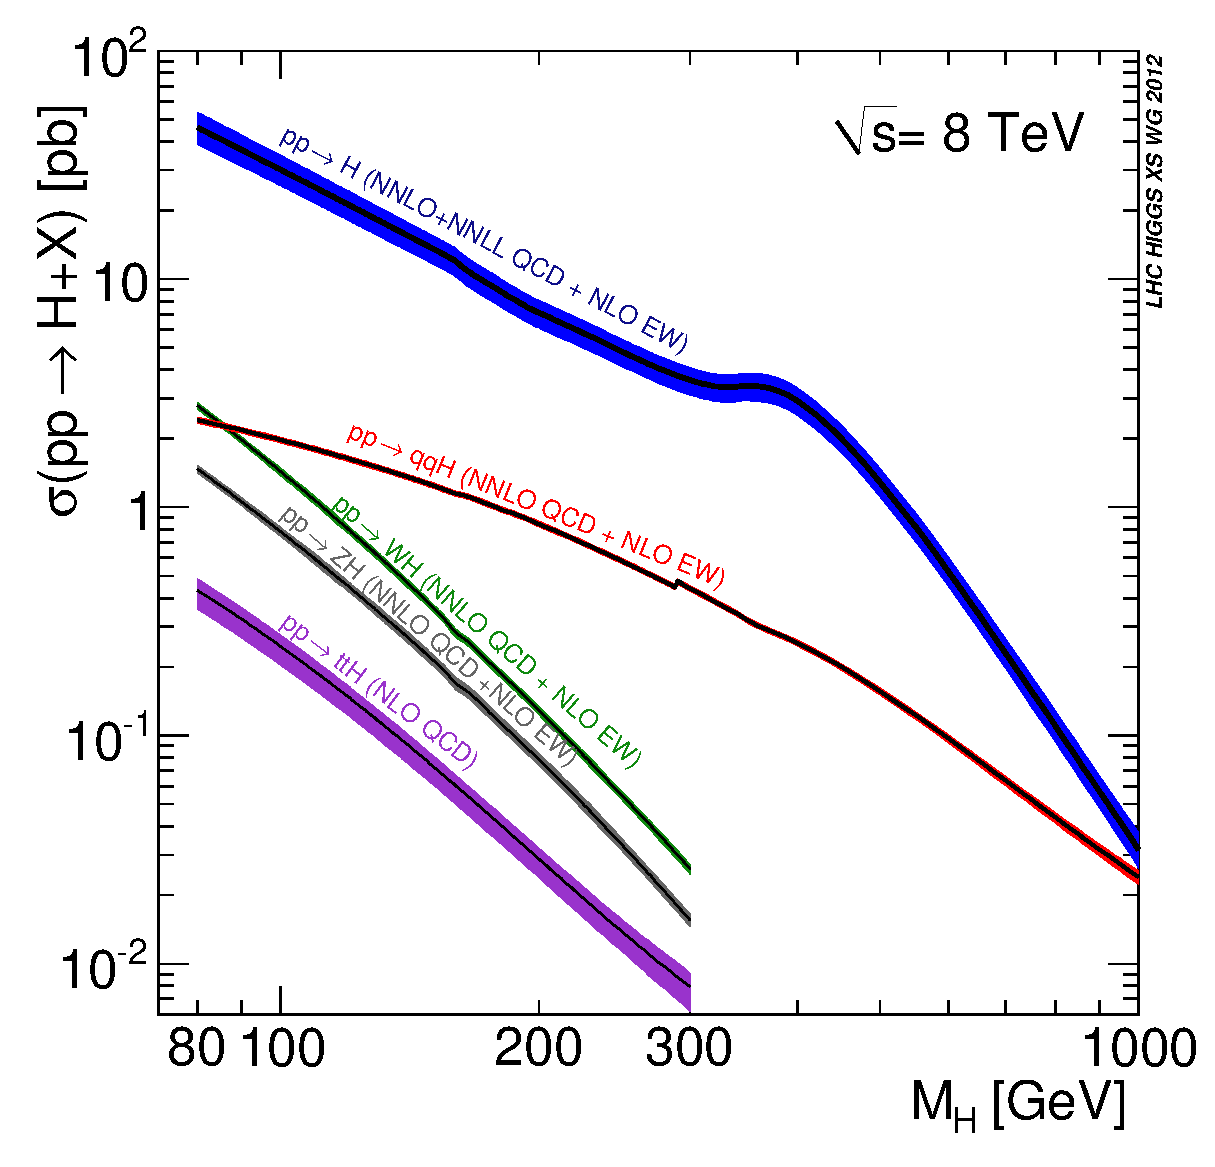
\includegraphics[width=0.48\textwidth]{tex/motivation/xs_fullrange}
	\caption{Cross sections for Higgs boson production versus mass for the low mass range (left) and an expanded mass range (right) \cite{YR2}. Theoretical uncertainties are also displayed. The blue band is \ac{ggF}, the red band is \ac{VBF}, the green band is \WH, the grey band is \ZH and the purple band is \ttH.}
	\label{fig:higgs_xs}
\end{figure}

The \ac{BR} of each decay channel is shown in \Figure~\ref{fig:higgs_br}, for a range of 
\mH. At a basic level, they are understood in terms of the Higgs coupling being 
proportional to mass and the kinematic requirement that $m_H > m_X + m_Y$ for 
\HepProcess{\PHiggs \HepTo XY} (accounting for off-shell decays).
The \HepProcess{\Pphoton \Pphoton}, \HepProcess{\PZ \Pphoton} and 
\HepProcess{\Pgluon \Pgluon} decay modes are different since they feature massless 
particles, and therefore proceed via loops of massive charged particles (electric charge 
for \HepProcess{\Pphoton \Pphoton} and \HepProcess{\PZ \Pphoton}, colour charge for 
\HepProcess{\Pgluon \Pgluon}).

It can be seen that the dominant decay channel for a low-mass (high-mass) Higgs boson is 
\HepProcess{\Pbottom \APbottom} (\WW). However, searches for 
\HepProcess{\PHiggs \HepTo \Pbottom \APbottom} are particularly challenging at hadron 
colliders owing to large backgrounds. In some cases (such as \WW and \ZZ), the decays of 
the decay particles themselves must be considered when designing an analysis.

\begin{figure}
	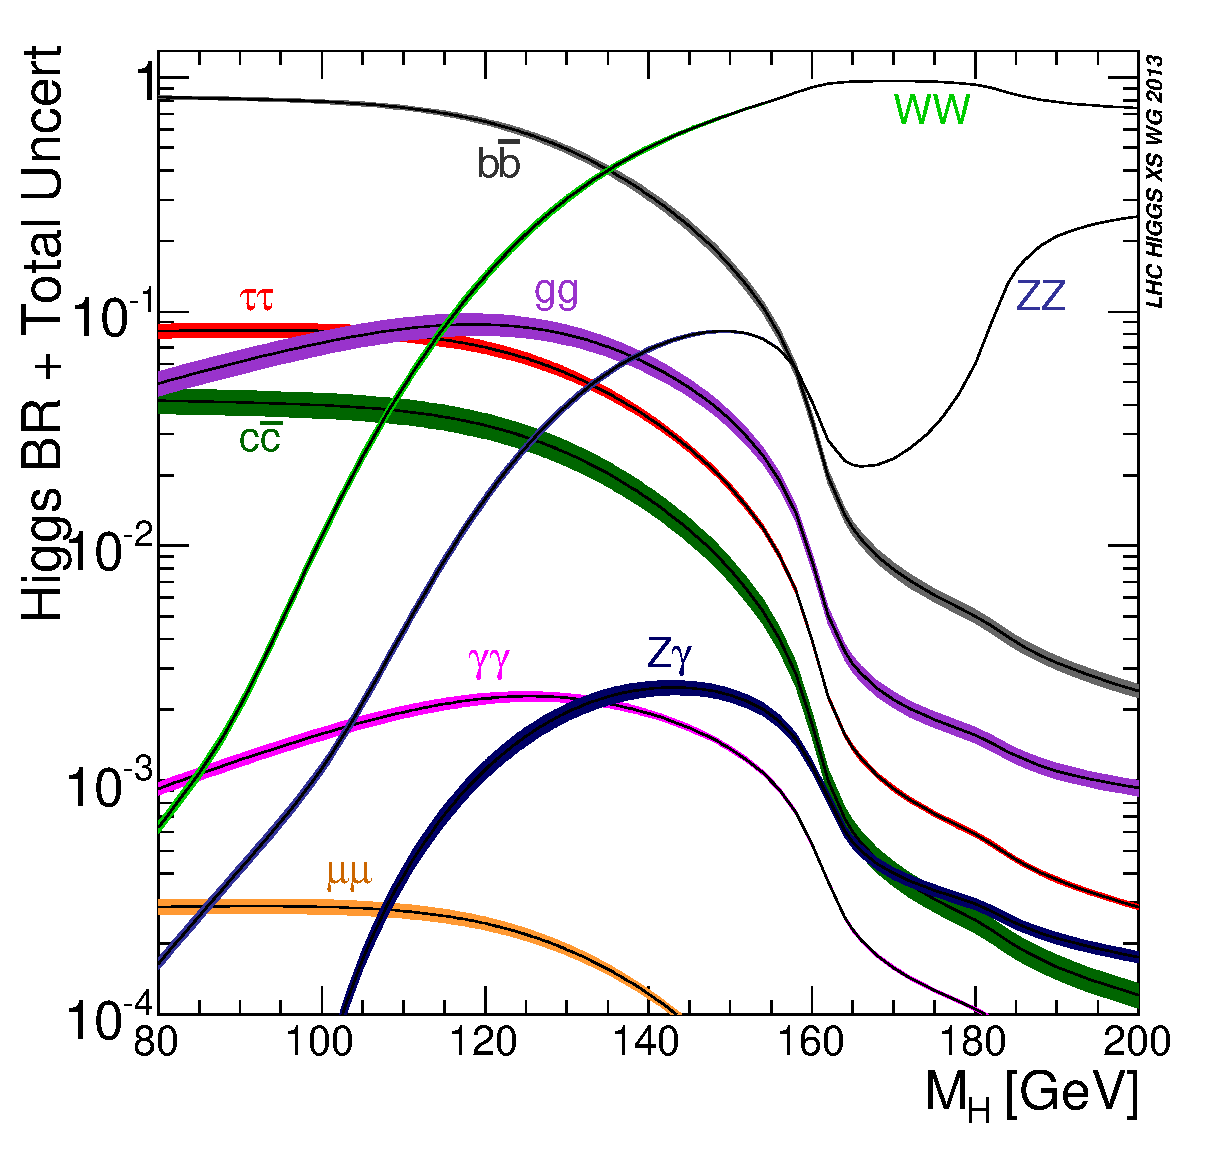
\includegraphics[width=0.48\textwidth]{tex/motivation/BR_lowrange}
	\hfill
	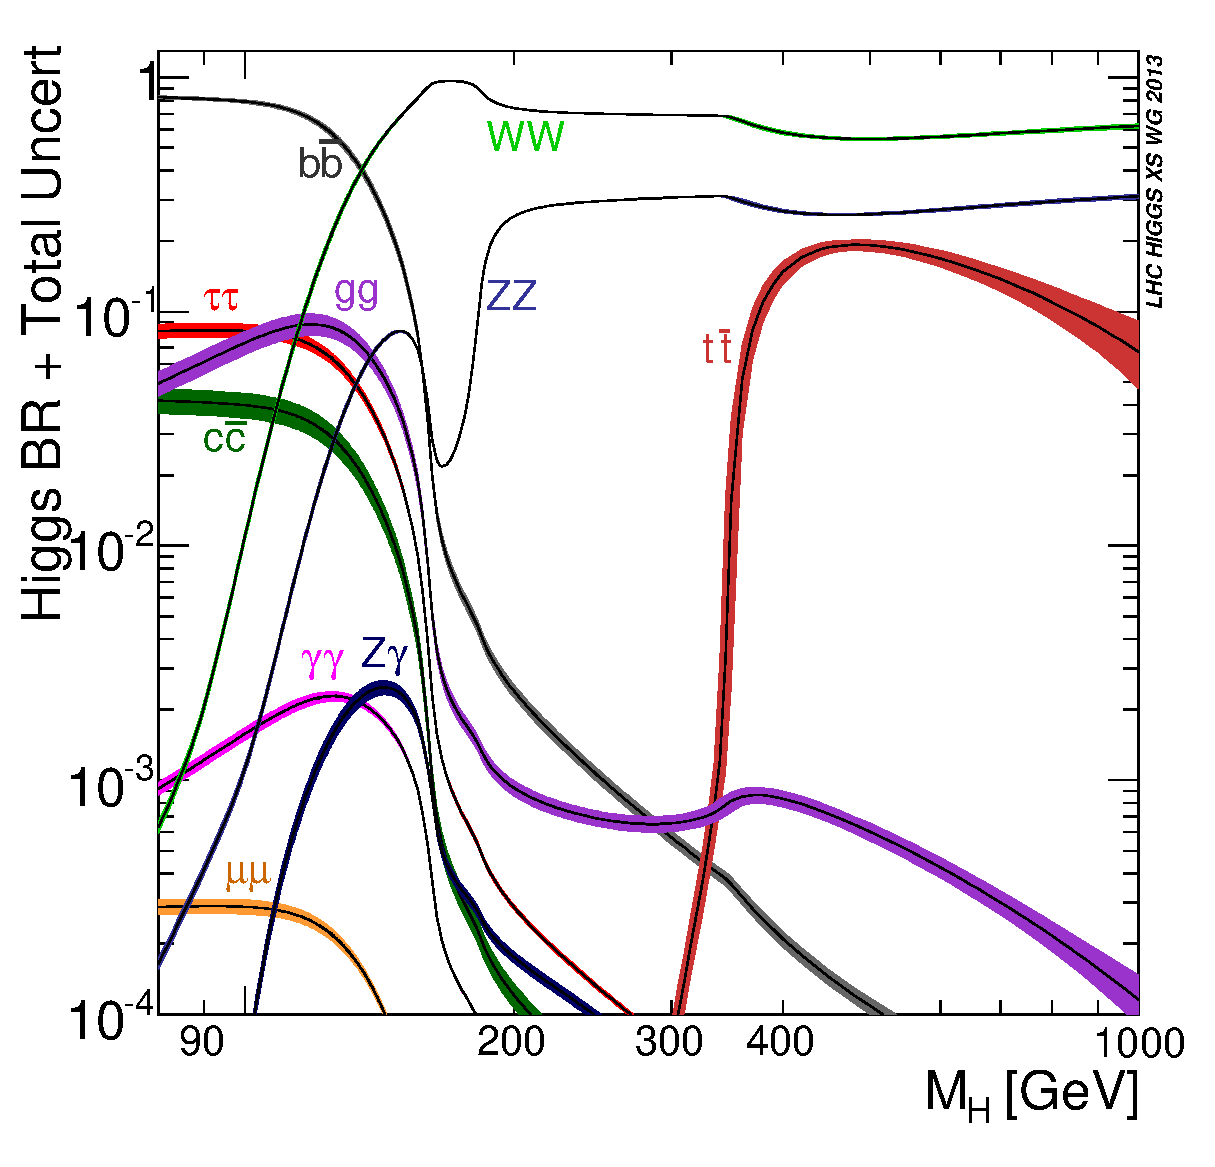
\includegraphics[width=0.48\textwidth]{tex/motivation/BR_fullrange}
	\caption{Branching ratios of the Higgs boson versus mass for the low mass range (left) and an expanded mass range (right) \cite{YR3}. Theoretical uncertainties are also displayed.}
	\label{fig:higgs_br}
\end{figure}
